%DO NOT ALTER THIS BLOCK OF COMMANDS.
\documentclass[12pt]{article}
\usepackage[margin=1in, bottom=4.5cm]{geometry}
\usepackage{amsmath,amsthm,amssymb,amsfonts, enumitem, fancyhdr, color, comment, graphicx, environ, scrextend, tikz, mathtools}
\pagestyle{fancy}
\setlength{\headheight}{65pt}
\newenvironment{problem}[2][Problem]{\begin{trivlist}
\item[\hskip \labelsep {\bfseries #1}\hskip \labelsep {\bfseries #2}]}{\end{trivlist}}
\newenvironment{lemma}[2][Lemma]{\begin{trivlist}
\item[\hskip \labelsep {\bfseries #1}\hskip \labelsep {\bfseries #2}]}{\end{trivlist}}
\newenvironment{theorem}[2][Theorem]{\begin{trivlist}
\item[\hskip \labelsep {\bfseries #1}\hskip \labelsep {\bfseries #2}]}{\end{trivlist}}
\newenvironment{proposition}[2][Proposition]{\begin{trivlist}
\item[\hskip \labelsep {\bfseries #1}\hskip \labelsep {\bfseries #2}]}{\end{trivlist}}
\newenvironment{corollary}[2][Corollary]{\begin{trivlist}
\item[\hskip \labelsep {\bfseries #1}\hskip \labelsep {\bfseries #2}]}{\end{trivlist}}
\newenvironment{sol}
    {\emph{Proof.}
    }
    {
    \qed
    }
\specialcomment{com}{ \color{blue} \textbf{Comment:} }{\color{black}} %for instructor comments while grading
\NewEnviron{probscore}{\marginpar{ \color{blue} \tiny Problem Score: \BODY \color{black} }}


\newcommand\restr[2]{{% we make the whole thing an ordinary symbol
  \left.\kern-\nulldelimiterspace % automatically resize the bar with \right
  #1 % the function
  \vphantom{\big|} % pretend it's a little taller at normal size
  \right|_{#2} % this is the delimiter
  }}
%%%%%%%%%%%%%%%%%%%%%%%%%%%%%%%%%%%%%%%

%%%%%%%%%%%%%%%%%%%%%%%%%%%%%%%%%%%%%%%%%%%%%
%Fill in the appropriate header information below
\lhead{Trey Manuszak \\ Christian Garcia}  %replace with your name
\rhead{MAT 445: Number Theory \\ 3/26 Lecture Notes}
%%%%%%%%%%%%%%%%%%%%%%%%%%%%%%%%%%%%%%%%%%%%%

%%%%%%%%%%%%%% PUT YOUR TITLE PAGE INFO HERE
\usepackage{blindtext}
\title{MAT 445: Number Theory}
\date{March 17, 2020}
\author{Trey Manuszak\\ Arizona State University}
%%%%%%%%%%%%%%



%%%%%%%%%%%%%%%%%%%%%%%%%%%%%%%%%%%%%%
%Do not alter this block.
\begin{document}


%%%%%%%%%%%%%%%%%%%%%%%%%%%%%%%%%%%%

%%%%%THIS IS WHERE YOU WILL BE DOING ALL OF YOUR WORK
%Copy the following block of text for each problem in the assignment.
\section{Introduction and Review}

\hspace{1em} In the previous chapter we were introduced to the concept of a totient. The totient uses the notation ”$\phi$” and is a function which computes the total amount of coprime numbers between $0$ and a number $N$, not including the number $N$. The numbers that are coprime to the number $N$ are set in a list with the notation $\Phi(N)$.

\section{Totients of Composite Numbers}

\hspace{1em} To compute the totient of composite numbers, the use of the Chinese remainder theorem is needed. Given an integer $x$, the following two conditions are equivalent.
\begin{itemize}
    \item $x \in \Phi(N)$, i.e., $0 \leq x < N$ and $\text{GCD}(x,N) = 1$;
    \item $0 \leq x < N$ and there exists $y$ such that $xy \equiv 1 \pmod{N}$. \cite[pg.178]{weissman_2017}
\end{itemize}

Similar to the $\sigma$ function, the totient function is multiplicative. Formally:

\begin{theorem}{7.9} \textbf{(The totient is a multiplicative function)} \textit{Let $d$ and $e$ be positive coprime integers. Then $\phi (de) = \phi (d) \phi (e)$}.
\end{theorem}

\begin{sol}
Let $x \in [0,de)$. Then solving $xy \equiv 1 \pmod{de}$ is equivalent to solving $xy \equiv [1,1] \pmod{[d,e]}$ by the Chinese Remainder Theorem. Thus, $x \in \Phi(de)$ if and only if $x$ has a multiplicative inverse $\pmod{d}$ and $\pmod{e}$. That is, $x \in \Phi(de) \Longleftrightarrow x \equiv [a,b] \pmod{[d,e]}$ for integers $a \in \Phi(d)$ and $b \in \Phi(e)$.

The Chinese Remainder Theorem gives an injective correspondence between $\Phi(de)$ and pairs $[a,b]$ in which $a \in \Phi(d)$ and $b \in \Phi(e)$. Therefore, $\phi(de) = \phi(d)\phi(e)$.
\end{sol}

\vspace{1em}

An example, which was provided in the lecture, was finding $\Phi(36)$. Using the fact that the totient is multiplicative, we can say that numbers which are in $\Phi(36)$ are the those which are congruent to members of $\Phi(9) \pmod{9}$ and to a member of $\Phi(4) \pmod{4}$. To find the total number of elements in $\Phi(36)$, which is $\phi(36)$, we multiply the amount of elements from $\Phi(9)$ and $\Phi(4)$. One can easily see that $$\Phi(9) = \{1,2,4,5,7,8\} \hspace{1em} \text{and} \hspace{1em} \Phi(4) = \{1,3\}.$$ If we let $M_{36}$ be the $4 \times 9$ matrix with entry $m_{ij} \coloneqq 36 \pmod{[i,j]}$, then we get $$M_{36} = \begin{pmatrix}
0 & 28 & 20 & 12 & 4 & 32 & 24 & 16 & 8 \\
9 & 1 & 29 & 21 & 13 & 5 & 33 & 25 & 17 \\
18 & 10 & 2 & 30 & 22 & 14 & 6 & 34 & 26 \\
27 & 19 & 11 & 3 & 31 & 23 & 15 & 7 & 35
\end{pmatrix}$$
So, by removing rows 0 and 2 and columns 0, 3, and 6, we get that $$\Phi(36) = \{1,29,13,5,25,17,19,11,31,23,7,35\}.$$
Also, since $\left| \Phi(9) \right| = 6$ and $\left| \Phi(4) \right| = 2$, then $\left| \Phi(36) \right| = \phi(36) = 12$.

\vspace{1em}

"I found Proposition 7.10 to be my favorite part of this chapter since it uses primes to compute $\phi(N)$, which I found to be interesting and efficient to compute the number of elements in the set $\Phi(N)$." - Christian Garcia



\begin{proposition}{7.10}
\textit{Let $p$ be a prime number, and let $e$ be a positive integer. Then, $\phi(p^e) = p^e - p^{e-1}$}.
\end{proposition}

\begin{problem}{7.11} Compute the totient $\phi(100)$.

\hspace{1em} \textit{Solution}: Using Proposition 7.10 to compute $\phi(100)$. We find that 
\begin{align*}
    \phi(100) &= \phi(2^2)\phi(5^2) \tag*{(By multiplicity of $\phi$)} \\ &= (2^2 - 2^1)(5^2 - 5^1) \tag*{(By Proposition 7.10)} \\ &= 2 \cdot 20 \\ &= 40. 
\end{align*}
\end{problem}

\section{Euler's Product Formula and Ideas}

\hspace{1em} This is also similar to Euler's product formula, which is not mentioned in the textbook and, generalized, goes as follows.

\begin{theorem}{7.24 (Euler's general product formula)} \textit{Suppose that $f(n)$ is a multiplicative function, and let $F(n) = \sum_{n = 1}^\infty f(n)/n^s$. If $s$ is a real number for which the series $F(s)$ is absolutely convergent, then for $\mathcal{P}$, the set of primes, we get} \begin{align*}
    F(s) = \prod_{p \in \mathcal{P}} \left( 1 + \frac{f(p)}{p^s} + \frac{f(p^2)}{p^{2s}} + \frac{f(p^3)}{p^{3s}} + \dots \right). \tag*{\cite[pg.381]{niven1991introduction}}
\end{align*}
\end{theorem}

\vspace{1em} The proof of this theorem will not be discussed, as it is beyond the scope of this course, but it can be applied to the $\phi$ function, as it is multiplicative.

\vspace{1em}

\begin{corollary}{7.25 (Euler's $\phi$-function product formula)}
\textit{Let $n \in \mathbb{Z}^+$ and $p$ prime. Then, } $$\phi(n) = n\prod_{p \mid n} \left( 1 + \frac{1}{p} \right).$$
\end{corollary}

\begin{problem}{7.26} Find $\phi(36)$ using the Euler $\phi$-function product formula.

\textit{Solution}: \begin{align*}
    \phi(36) &= \phi(2^23^2) \\ &= 36(1 - \frac{1}{2})(1 - \frac{1}{3}) \\ &= 36 \cdot \frac{1}{2} \cdot \frac{2}{3} \\ &= 12.
\end{align*}
\end{problem}

Another interesting result can be seen in the figure at the bottom of page 181, where Weissman graphs $\phi(n)/n$. \cite[pg.181]{weissman_2017} Attempting a different interesting graphic, consider the following depiction of the reciprocal.

    \begin{center}
    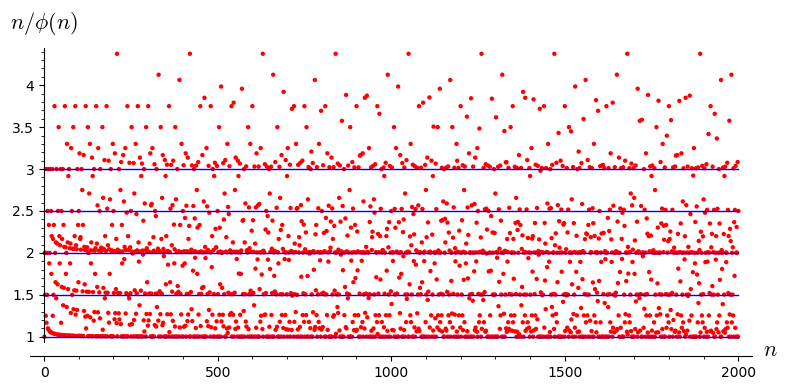
\includegraphics[scale=.5]{plot445 (1).png}
    \end{center}
One can see the convergence of points on the half integers, which is emphasized in blue. One might ask if as $n$ gets larger, do we see this convergence on every half integer? This may also tend to raise the analysis question if $\lim_{N \to \infty} \frac{1}{N}\sum_{n = 1}^N \frac{n}{\phi(n)} = \frac{\pi^2}{6}$.

\section{Totients of Composite Numbers Cont.}

\hspace{1em} As stated in the book, multiplicative inverses can be lifted up a tower of prime powers. In other words, if $p$ is prime, then $\text{GCD}(x,p) = 1$ if and only if $\text{GCD}(x,p^e) = 1$ for all positive exponents $e$. A way to lift a multiplicative inverse$\pmod{p}$ is achieved by applying the following lemma. \cite[pg.183]{weissman_2017}

\begin{lemma}{7.16 (Lifting multiplicative inverses)} \textit{Suppose that $xy \equiv 1 \pmod{p^e}$. Define } $$z = y - yrp^e.$$ \textit{Then $xz \equiv 1 \pmod{p^{2e}}$}.
\end{lemma}

\vspace{1em}

In a similar, yet more precise manner, one can take the idea of lifting multiplicative inverse up into higher prime powers and translate it to square roots.

\begin{theorem}{7.20 (Lifting square roots)}
\textit{Suppose that $p$ is an odd prime, $e \geq 1$, $\text{GCD}(a,p) = 1$, and $x^2 \equiv a \pmod{p^e}$. Let $r$ be the integer for which $x^2 = a + rp^e$. Let $b$ be a multiplicative inverse of $2x$, modulo $p^e$. Define} $$z = x - brp^e.$$ \textit{Then $z^2 = a \pmod{p^{2e}}$}.
\end{theorem}

\vspace{1em}

For those familiar with Ring Theory, this can be generalized to polynomials with coefficients in an integral domain as follows.

\begin{theorem}{7.27 (Hensel's Lemma)} \textit{Suppose that $f(x)$ is a polynomial with integral coefficients. If $f(a) \equiv 0 \pmod{p^j}$ and $f'(a) \not\equiv 0 \pmod{p}$, then there is a unique $t \pmod{p}$ such that $f(a+tp^j) \equiv 0 \pmod{p^{j+1}}$.} \cite[pg.87]{niven1991introduction}
\end{theorem}

\vspace{1em}

So, since $\mathbb{Z}$ is an integral domain and considering all polynomials of degree zero, like before, we can show that if the polynomial has a simple root$\pmod{p}$, which doesn't just need to be root two, then it has a unique root in a higher power of $p$.

\section{RSA Public-Key Cryptosystem}

\hspace{1em} Also covered in the book, was the topic of the RSA public key cryptosystem. To lay down the idea of the RSA cryptosystem, consider the following scenario. Alice wants to send the text "B" to Jake. For simplicity sake, we'll let each letter we want to send be translated to it's position in the alphabet. So, Alice wants to send the text "2" to Jake. Jake's public key, which is know to everybody, is the pair $(17,22)$. So, we get the following encryption, \begin{align*}
    2^{17} \pmod{22} &= 131072 \pmod{22} \tag*{(Note "2" is the text we are encrypting)} \\ &= 18 \pmod{22}.
\end{align*}
So, what is getting received by Jake, and for any malicious receivers, is the 18th letter "r", which is called the \textbf{ciphertext}. This text is encrypted and looks pseudorandom to anyone without the private key to decrypt the message. Now, Jake is going to use his private key, which no one knows the contents of, which for the sake of the scenario is $(23,22)$. To unlock the text, Jake will do the following calculation, \begin{align*}
    18^{23} \pmod{22} = 2 \pmod{22}.
\end{align*}
Doing the calculation, Jake found the text to read "2", or "B" just as planned.

Now how does this work? First, Jake selected two prime numbers, $p = 2$ and $q = 11$. Then, multiply them together to get $N = 22$. Next, we compute $\phi(N) = 10$. Then, we choose $e$ such that $1 < e < \phi(N)$ and $e$ is coprime with $N$ and $\phi(N)$. Jake chose $e = 17$. This gave us the public key $(e,N)$, or $(17,22)$ in the scenario. Lastly, choose $d$ such that $de \pmod{\phi(N)} = 1$. Jake chose $d = 23$. This gives us the private key $(d,N)$, or $(23,22)$ in the scenario. The larger the primes chosen at the beginning of the process, the decryption becomes near impossible for people trying to intercept the messages.

\section{NTRUEncrypt Public-Key Cryptosystem}

\hspace{1em} Lastly, covered in the lecture, was the topic of NTRUEncrypt public key cryptosystem. By letting $\vec{h}(x) = h_0 + h_1x + \dots + h_{N-1}x^{N-1}$ be an NTRUEncrypt public key, then you get the NTRU lattice $L_{\vec{h}}^{NTRU}$ that is associated with $\vec{h}(x)$, which is the $2N$-dimensional lattice spanned by the rows of the matrix 
%\[ INCASE THE BELOW DOESNT WORK ANYMORE
%    M_{\vec{h}}^{NTRU} = \left(
%    \begin{array}{cccc|cccc}
%      1 & 0 & \dots & 0 & h_0 & h_1 & \dots & h_{N-1}\\ %row1
%      0 & 1 & & & h_{N-1} & h_0 & \dots & h_{N-2} \\ %row2
%      \vdots & & \ddots & & \vdots & \vdots & \ddots & \vdots \\ %row3
%      0 & & & 1 & h_1 & h_2 & & h_0 \\ %row4
%      \hline
%      0 & \dots & & 0 & q & 0 & \dots & 0 \\ %row5
%      \vdots & \ddots & & & 0 & q & & \\ %row6
%      & & & & \vdots & & \ddots & \\ %row7
%      0 & & & 0 & 0 & & & q
%    \end{array}
%    \right)
%  \]
  
  \[
    M_{\vec{h}}^{NTRU} = \left(
    \begin{array}{cccc|cccc}
      1 & & & \hspace{-2mm}\raisebox{-1ex}[0ex][0ex]{\makebox(0,0){\text{\huge0}}} & h_0 & h_1 & \dots & h_{N-1}\\ %row1
      & 1 & & & h_{N-1} & h_0 & \dots & h_{N-2} \\ %row2
      & & \ddots & & \vdots & \vdots & \ddots & \vdots \\ %row3
      \raisebox{2ex}[0ex][0ex]{\makebox(0,0){\text{\huge0}}} & & & 1 & h_1 & h_2 & & h_0 \\ %row4
      \hline
      & & & & q & & & \raisebox{-2ex}[0ex][0ex]{\makebox(0,0){\text{\huge0}}} \\ %row5
      & & & & & q & & \\ %row6
      & &\hspace{-4.5mm}\raisebox{2ex}[0ex][0ex]{\makebox(5,0){\text{\huge0}}} & & & & \ddots & \\ %row7
      & & & & \raisebox{2ex}[0ex][0ex]{\makebox(0,0){\text{\huge0}}} & & & q
    \end{array}
    \right),
  \]
which can be abbreviated by \begin{align*}
    M_{\vec{h}}^{NTRU} = \begin{pmatrix}
    I & \vec{h} \\
    0 & qI
    \end{pmatrix}.
\end{align*}

One can further reference key creation, encryption, and decryption from the lecture notes written by Hoffstein, Pipher, and Silverman. \cite{hoffstein1998ntru} Now, one might wonder what the benefit of the NTRUEncrypt cryptosystem is. Well, encryption and decryption takes $\mathcal{O}(N^2)$ time in NTRUEncrypt and $\mathcal{O}(N^3)$ time in RSA for a block of length $N$. So, it is much faster to use NTRUEncrypt. Further, the NTRUEncrypt key lengths are $\mathcal{O}(N)$ compared to an RSA key length of $\mathcal{O}(N^2)$. Thus, not only is NTRUEncrypt faster, it takes up less memory. Also, while it isn't completely known yet, many researchers believe NTRUEncryption will be more secure in the quantum computing era than RSA or Elliptic Curve encryption.
\newpage
\medskip

\bibliographystyle{unsrt}
\bibliography{sample}

%%%%%%%%%%%%%%%%%%%%%%%%%%%%%%%%%%%%%%%%
%Do not alter anything below this line.
\end{document}